\chapter{Related Work} % Main chapter title

\label{related_work} % For referencing the chapter elsewhere, use \ref{Chapter2}

\section{Transformer}
\label{sec:rel_transformer}

Transformer models have revolutionized how sequential data is processed in deep learning. 
Introduced by Vaswani et al. (2017) in the foundational paper “Attention Is All You Need” 
\cite{attention}
, the Transformer architecture relies entirely on attention mechanisms instead of recurrence or convolution.
This design enables parallel processing of sequence elements and captures long range dependencies 
more effectively than previous recurrent neuronal network (RNN)-based approaches. 
At its core, a Transformer uses a mechanism called self-attention to weigh the importance of different 
tokens (elements) in a sequence relative to one another, 
allowing the model to focus on relevant context regardless of its positional distance. 
This ability to draw global dependencies between input and output makes Transformers powerful 
for tasks like machine translation, where the entire input sequence informs each output element. 

\begin{marginfigure}[] % move figure up by 1 line -5\baselineskip
    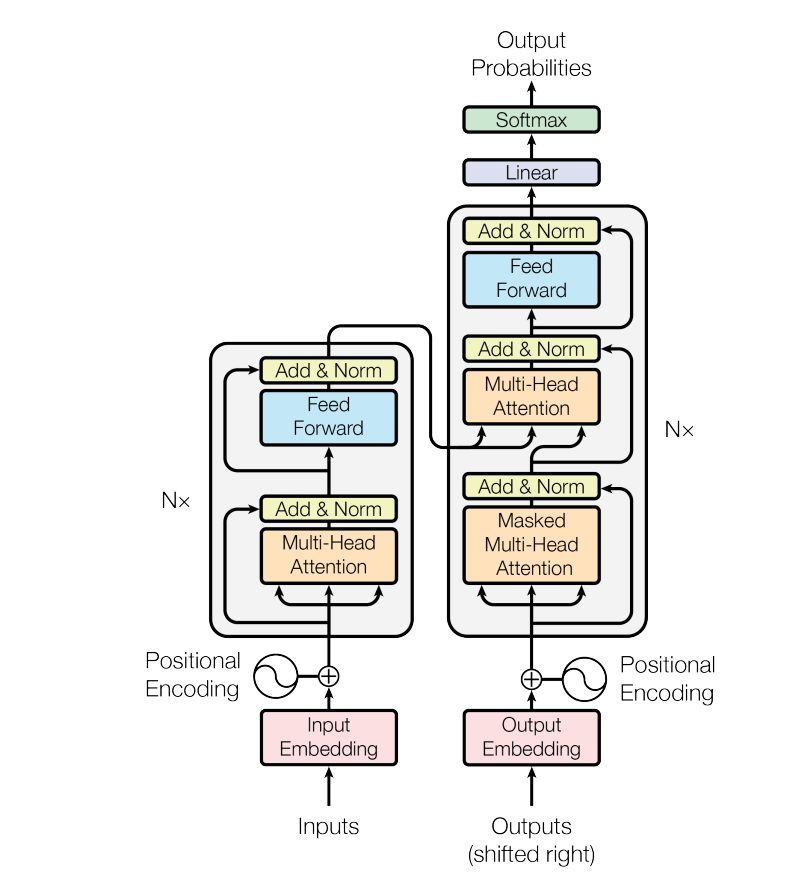
\includegraphics[width=1\marginparwidth]{2_RelatedWork/attention.png}
    \caption{\label{fig:malratios}
    Taken From \cite{attention}}
\end{marginfigure}

In a self-attention layer, the model computes attention scores between every pair of tokens in a sequence. 
Each token is first converted into an embedding vector, by looking up the token in the embedding matrix
with the dimensionality (vocabulary size, hidden size). 
The embedding vector has a length of "hidden size".
From each embedding vector then a Query, Key, and Value vector is derived via multiplication with learned 
projection matrices.
Next attention scores are obtained by comparing Queries against Keys via a dot product. 
These scores determine how much attention one token should pay to another when constructing 
its next representation. 
After a softmax normalization layer, each token Value vector aggregates information from all 
other tokens Value vectors, weighted by these attention scores.
Finally, this weighted sum of Value vectors produces a new contextualized embedding for that token, 
capturing relationships between words dynamically.
Transformers employ multi-head attention, meaning this process is replicated in parallel multiple times 
(with different learned projection matrices). 
Multi-head attention allows the model to attend to different patterns or aspects of the data simultaneously, 
capturing different kinds of relationships in the sequence. 
The outputs of multiple heads are then combined, 
enabling richer representations than a single attention operation. 
Because the Transformer has no recurrent notion of sequence order, 
it adds positional encodings to token embeddings to inject information about each tokens position 
in the sequence.

The original Transformer architecture is an encoder-decoder model, 
consisting of a stack of encoder layers and a stack of decoder layers
\cite{attention}
. Each encoder layer has two main sublayers: 
a multi-head self-attention sublayer that allows each input token to attend to others, 
and a feed-forward network sublayer that further transforms each tokens representation 
(each sub-layer is wrapped with residual connections and layer normalization for stability). 
Stacking multiple such layers produces an encoder that maps an input sequence into a sequence of 
high level feature vectors.
On the other side of the encoder-decoder, each decoder layer also contains 
a self-attention sublayer (applied to the decoders own inputs generated so far) and 
a feedforward sublayer, 
but additionally includes an encoder-decoder attention sublayer (also called cross-attention). 
This cross-attention allows the decoder to attend to the encoders output at each decoding step, 
effectively using the encoded source sequence context when predicting each token. 
The decoder generates one output token at a time, 
and each token embedding can only attend to earlier 
token embeddings (preventing a token from “seeing” future tokens during training). 
This encoder-decoder design proved extremely effective for sequence-to-sequence tasks like 
neural machine translation, 
where the encoder processes an input sentence into a context representation and 
the decoder generates an output sentence using that context \cite{deep_translate, gtrans}.


\begin{marginfigure}[] % move figure up by 1 line -5\baselineskip
    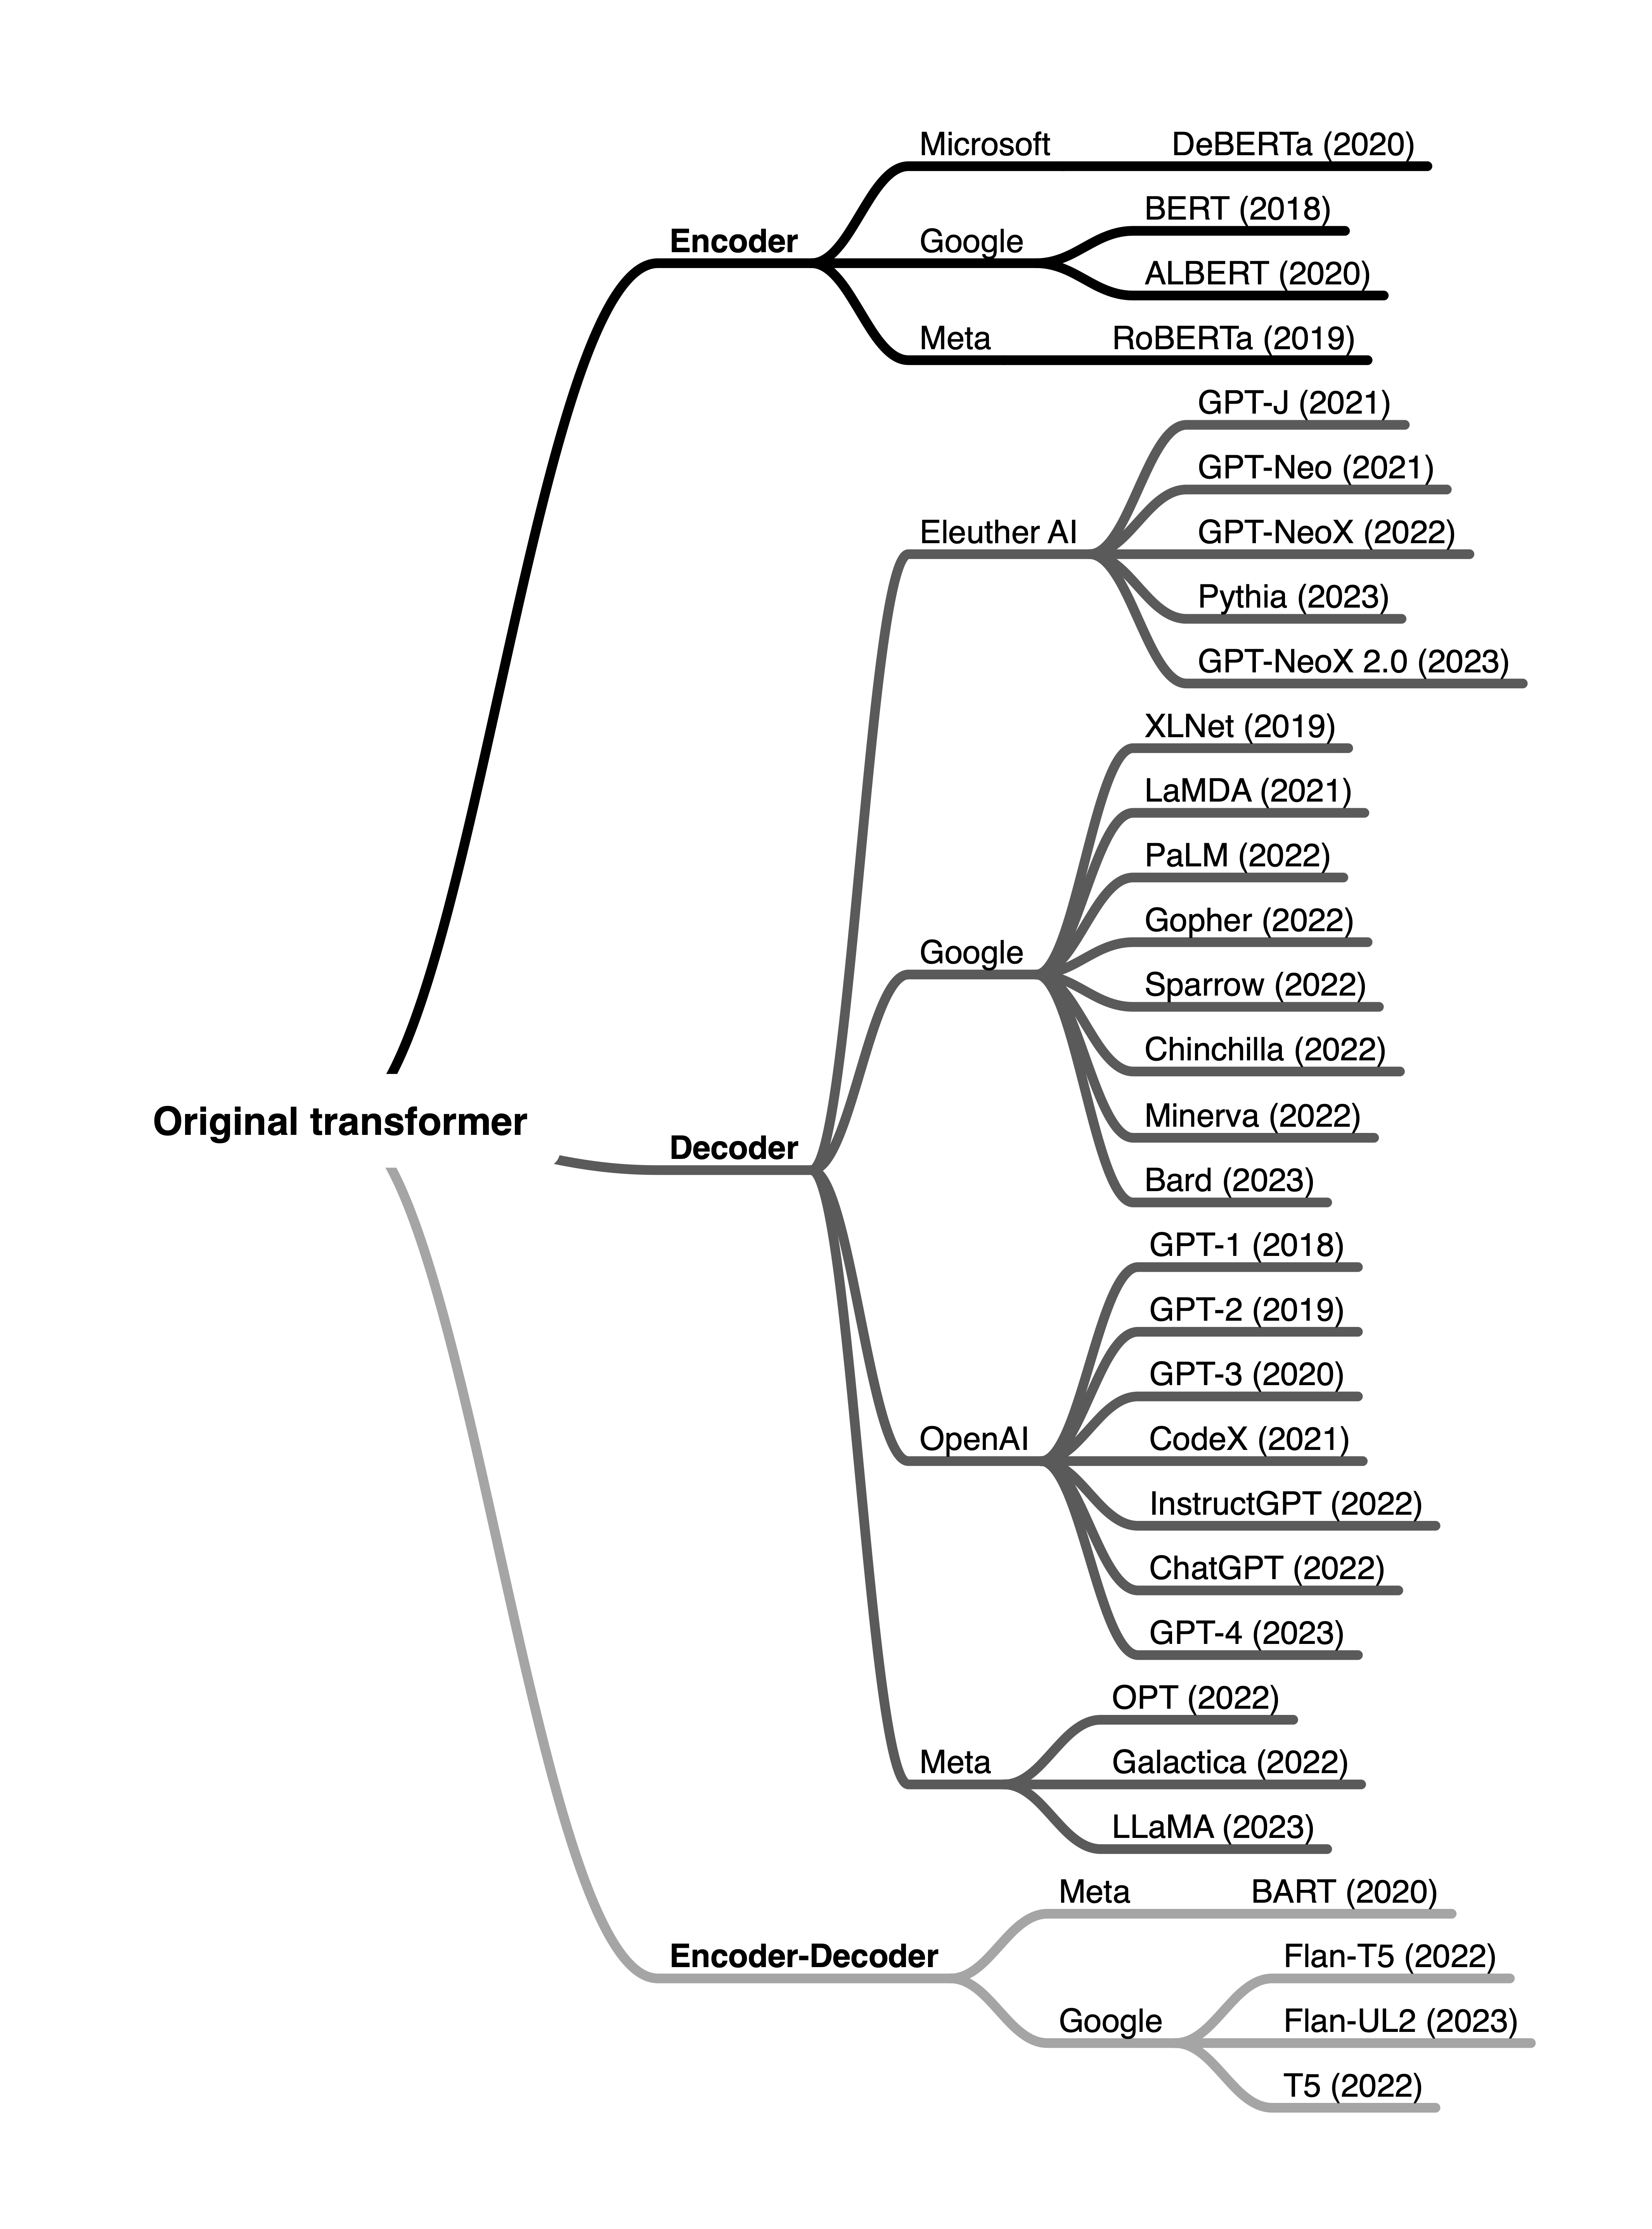
\includegraphics[width=1\marginparwidth]{2_RelatedWork/transformer_variants.png}
    \caption{\label{fig:malratios}
    Taken From https://magazine.sebastianraschka.com/p/understanding-encoder-and-decoder}
\end{marginfigure}

While the original Transformer uses both an encoder and a decoder, 
many modern applications use only one of the two stacks, depending on the task. 
An encoder only Transformer (just the stack of self-attention and feed-forward layers) 
is well suited for producing a fixed length embedding of an input e.g. for classifying it. 
Bidirectional Encoder Representations from Transformers (BERT) \cite{bert} is a popular example: 
it directly outputs contextualized embeddings from the top encoder layer to be used for prediction tasks. 
In contrast, decoder only Transformers (also called "autoregressive Transformers") 
use just the decoder mechanism to generate sequences. 
These models, exemplified by the GPT series \cite{gpt1, gpt2, gpt3, gpt4}, 
model probability distributions over sequences by predicting each next token given the previous ones. 
In essence, encoder only Transformers encode a full sequence to an embedding 
(useful for understanding or classification), 
whereas decoder only Transformers decode/generate a sequence one token at a time 
(useful for language modeling). 
Both styles share the same self-attention building blocks, 
with differences mainly in whether they process an input sequence as a whole (encoders) 
or produce an output sequentially (decoders). 

One of the biggest breakthroughs following the original Transformer \cite{attention} 
was the introduction of BERT by Devlin et al. in late 2018 \cite{bert}. 
BERT uses the Transformer encoder only architecture to learn deep Bidirectional Encoder from Transformer 
of language.
In BERTs pretraining, some tokens in the input are masked at random and the model must predict 
these missing tokens (Masked Language Modeling), 
and it also learns to predict if one sentence naturally follows another (Next Sentence Prediction). 
Through this process, BERT learns contextual embeddings that capture subtle relationships in language, 
as each tokens representation is influenced by the tokens on both its left and right. 
This bidirectional conditioning (as opposed to the one directional nature of a decoder) 
enabled BERT to achieve better performances on a wide range of NLP tasks once finetuned \cite{scoreBERT}.

Since "Attention Is All You Need", Transformer architectures have undergone numerous enhancements 
and spawned many variants. 
Early on, researchers scaled Transformers to larger sizes and data 
(e.g., Llama 2 \cite{llama2}, Llama 3 \cite{llama3} for text generation) and created optimized versions of BERT 
(such as RoBERTa \cite{roberta}, ALBERT \cite{albert}, and DistilBERT \cite{distilbert}) 
to improve training effectiveness or model efficiency. 
A major focus has been on addressing the quadratic complexity of standard self-attention with respect 
to sequence length \cite{nystromformer}. 
Vanilla Transformers compute attention between all pairs of $n$ tokens, 
which scales with $O(n^2)$ in time and memory. 
This becomes a problem for long sequences like lengthy documents or code analysis 
(e.g., an entire mobile apps code can consist of thousands of tokens). 
Starting around 2020, new and more efficient Transformers emerged to tackle this limitation.

Beltagy et al. introduced Longformer \cite{longformer}, 
which implements a sparse attention pattern to handle long text efficiently. 
Instead of each token attending to all others, 
Longformer restricts attention to a local window around each token and selectively uses a few 
global tokens. 
This combination allows the model to capture local context while still communicating information globally 
through the special tokens. 
By limiting the attention range, Longformer can process sequences up to 
4000 tokens with less than quadratic cost. 

BigBird \cite{bigbird}, introduced by Zaheer et al., 
takes a similar sparse attention approach. 
It mixes local attention, random attention, and a handful of global tokens to ensure every token can 
at least indirectly attend to every other token. 
BigBird can also handle sequences of up to 4000 tokens with manageable computation.
Both Longformer and BigBird reported that by limiting attention to only a subset of tokens 
(rather than all pairs), 
Transformers can scale to long sequences without sacrificing too much performance.

Another approach is Nyströmformer \cite{nystromformer} by Xiong et al. 
that applies the Nyström method (a technique for matrix approximation) to the self-attention computation.
Instead of computing the full $n \times n$ attention matrix, 
Nyströmformer samples a set tokens and uses them to construct an approximate attention matrix 
at only O(n) cost. 
This approximation allows the model to scale linearly with sequence length, 
a big improvement in efficiency. 
Nyströmformer reports competitive accuracy on many NLP tasks compared to 
standard Transformer, despite using only a fraction of the computation. 
This kind of efficient attention is especially relevant for resource constrained settings. 
For instance, the recent DetectBERT \cite{detectbert} approach for Android malware analysis 
leveraged a Nyströmformer layer to handle a large amount of Embeddings at once 
(more details in section \ref{sec:detectbert}). 
By using Nyströmformer, DetectBERT reports to process each app in a single forward pass (up to ~8000 tokens) 
with only ~2 GB of GPU memory, achieving inference times on the order of 5 milliseconds per app. 

Researchers have also revisited the classic BERT model to incorporate recent advancements, 
leading to the development of ModernBERT.
ModernBERT extends the native input length to 8000 tokens, overcoming BERTs original 512-token limit. 
It also incorporates optimization techniques from the Transformer research of the past few years 
(such as improved training regimes, more efficient attention implementations, 
and better normalization methods). 
Trained on an 2 trillion token corpus, ModernBERT achieves SOTA results across a wide array of 
classification and retrieval tasks (including domains like long text and code). 
Impressively, these gains seem come without tradeoffs in practicality.
ModernBERT is faster and more memory-efficient than older encoders and is still 
running inference on common GPUs.

\section{Malware Detection}

Malware detection approaches include static, dynamic, and network-based methods \cite{vorlesung}.
While this thesis focuses on static analysis, it is worth briefly noting the other approaches for context.
Static analysis examines APK features such as source code and binaries without executing the app.
This makes it highly scalable and suitable for large-scale evaluations.
Prior research like \cite{drebin} and \cite{detectbert} demonstrate the effectiveness and efficiency of static approaches.
However, static analysis does face challenges, including evasion techniques like code obfuscation and polymorphism.
Dynamic analysis, in contrast, observes malware behavior at runtime.
Although it provides richer contextual insights, it requires significant resources and infrastructure and is vulnerable to other evasive strategies, such as sandbox detection.
Similarly, network analysis examines communication patterns and data flows to identify malicious activity.
Hybrid techniques that integrate these methods aim to combine their strengths while mitigating individual limitations.
These, too, face challenges such as computational complexity and integration difficulties.
This thesis, therefore, focuses solely on static analysis as a scalable and efficient approach for malware detection.

Malware authors often employ evasion techniques to bypass detection mechanisms \cite{vorlesung}.
In static analysis, common strategies include manipulating code structures through obfuscation \cite{obfuscation} and polymorphism \cite{polymorhism}.
Obfuscation involves transforming code into a more complex or less readable form to conceal its true purpose, whereas polymorphism allows malware to dynamically change its appearance while maintaining its core functionality.
These approaches exploit the limitations of analyzing code without running it.
While dynamic and network based methods address some of these weaknesses, they introduce their own vulnerabilities, such as susceptibility to sandbox detection and reliance on communication pattern anomalies.
Transformers ability to handle obfuscation and learn robust representations of static code helps mitigate some of these challenges \cite{deobfuscation}.

Concept drift refers to the gradual evolution of malware patterns, which often leads to a decline in the performance of detection models over time.
Models like Transcend \cite{transcend} have tackled this issue by introducing mechanisms to detect and adapt to concept drift during deployment.
However, these methods are resource-intensive and may struggle to generalize across diverse datasets.
Addressing concept drift remains a critical challenge for static Android malware detection and is one criteria used in this thesis.
Some works have proposed automated drift detectors that trigger model updates when the 
input data distribution shifts
\cite{morph}

\subsection{Android Malware Detection}
\label{sec:amd}
Detecting malware on the Android platform presents unique challenges and opportunities due to its open ecosystem and the high volume of apps and malware samples. The availability of many labeled datasets such as Androzoo, Drebin, Transcend, and DexRay has driven research in this domain.

Drebin \cite{drebin} represents a leap in Android malware detection, being both a dataset and an approach. 
As an SVM-based method, Drebin achieves remarkable results, significantly outperforming other 
approaches by detecting 94\% of malware samples at a false-positive rate of just 1\%. 
This demonstrated the high effectiveness of machine learning-based static Android malware detection, 
striking a balance between accuracy and efficiency. 
The Drebin dataset itself provides labeled malware samples with rich the APK files of each Android 
application being provided, making it a foundational resource in the field.

Transcend \cite{transcend}, on the other hand, introduced the critical concept of drift into 
Android malware detection.
It highlights how models trained on older datasets like Drebin experience performance decay when 
applied to newer, evolving datasets.
This evolution in malware characteristics, known as concept drift, underscores the need 
for adaptive retraining mechanisms.
Transcend serves as a benchmark for evaluating the robustness of detection models over time 
and emphasizes the importance of building systems that can sustain detection accuracy in the 
face of changing malware landscapes.

DexRay \cite{dexray} is as well a model and a dataset comprising 158,803 Android applications, 
including both benign and malicious samples, curated from AndroZoo. 
The dataset spans applications from 2019 to 2020, with benign apps defined as those not flagged 
by any antivirus on VirusTotal and malware apps identified by at least two antivirus engines. 
A distinguishing feature of the DexRay dataset is its explicit inclusion of both non-obfuscated 
and obfuscated applications, allowing researchers to assess the impact of code obfuscation on 
malware detection models. Given its large-scale and diverse composition, 
DexRay provides a valuable benchmark for evaluating detection techniques and analyzing how 
Android malware evolves over time.

Androzoo \cite{androzoo} is a comprehensive repository containing millions of APKs sourced 
from various app stores and spanning over a decade of Android app development.
The dataset provides significant scale and diversity, enabling researchers to analyze trends 
in malware evolution and assess the effectiveness of detection methods over time.
In addition to the APKs there was work done on mining metadata for the APKs, enabling further 
research on the landscape of Android Apps.


\section{Transformer based malware detection}

Recent research in cybersecurity has produced a range of Transformer based models for malware detection.
Many of these novel approaches build on the BERT 
\cite{bert} 
architecture or its variants, 
adapting them to capture the semantics of malicious code and improve detection performance. 
For example, MalBERT 
\cite{malbert}
uses a BERT variant that is finetuned on Android app manifest files for static analysis. 
By treating an apps manifest (which lists permissions, components, etc.) as input text, 
MalBERT achieved excellent results, with about 97\% accuracy and an F1 score around 95\% 
in distinguishing malware from benign apps, even when reproduced by other authors 
\cite{malbert_reproduce}. 
Its success indicates that Transformers can leverage even simple limited textual features (like manifests) 
for malware detection. 
However, focusing only on manifest content may miss code level clues e.g. 
obfuscated or malicious code could be overlooked if not reflected in the manifest. 
To address this, a followup model MalBERTv2 
\cite{malbert_two} 
extended the approach to be code-aware. 
MalBERTv2 processes actual app code by extracting the most informative code files and applying a 
custom tokenization before using a BERT based model.
This richer static analysis led to improved performance across multiple datasets: 
MalBERTv2 reports an F1 score of 97\% when evaluated on a mix of Android malware datasets.
On smaller subsets, MalBERTv2s F1 score ranged from about 82\% up to 94\%. 
These BERT based detectors demonstrate the Transformers ability to learn meaningful features from 
app data (manifest or code), resulting in high precision and recall. 
A limitation is that their large size (e.g. BERT base with 110 million parameters) can be expensive to execute. 

Purely codebased is another approach called DetectBERT \cite{detectbert}.
DetectBERT is a transformer based approach to Android malware detection that 
builds upon DexBERT \cite{dexbert}, 
another transformer based model designed for smali class level analysis of Android Smali code.
Using a Correlated Multiple Instance Learning (c-MIL) framework, 
DetectBERT aggregates Smali class embeddings of DexBERT into an app level representation.
The DetectBERT model is further analyzed in Chapter \ref{sec:detectbert} where it is evaluated as baseline.

Another recent model, BERTroid 
\cite{bertroid}
, further showcases Transformers potenital in Android malware detection. 
BERTroid is based on a BERT architecture and integrates neural embeddings from both static and dynamic 
analysis to classify apps. 
It was evaluated on several public datasets. 
BERTroid is reports to outperform prior SOTA solutions, achieving near perfect detection rates 
for instance, an Accuracy of 99.74\% and F1-score of 99.87\% on one benchmark, 
with precision and recall also around 99.87\%. 
Such results indicate a very high true positive and true negative rate. 
The authors note BERTroids resilience against concept drift, 
claiming it maintains high performance even as malware characteristics change over time. 
This hints that training on diverse and up to date data empowered the model to be robust to concept drift. 
It should be noted, however, that achieving nearly 99\%+ 
accuracy in malware detection can sometimes be a sign of evaluation on simplified scenarios 
real world deployment may see lower numbers due to novel malware samples or adaptive attackers. 
Nonetheless, BERTroid underscores the effectiveness of Transformer encoders in this domain. 

Similarly, Liu et al. propose SeMalBERT 
\cite{semalbert}
, which focuses on learning semantic representations of code using BERT. 
SeMalBERT achieved high detection rates, with accuracy improving from about 88.6\% up to ~98.75\%. 
This suggests that capturing semantic meaning makes the detector more robust to code obfuscation 
and variants, since semantically similar malware will be clustered in the Transformers feature space 
even if their surface syntax differs. 
Roziere et al. showed that pretrained Transformers can deobfuscate code and 
recover its functionality to an extent 
\cite{deobfuscation}
, underscoring the potential for resilience against obscured or polymorphic code. 
One key advantage is their ability to learn deep, contextual representations of code and API usage, 
which helps in resisting many common obfuscation techniques. 
Traditional static detectors often rely on specific keywords, signatures, or simple features that 
malware authors can easily obfuscate (e.g., renaming variables, reordering code, ...).
Transformers, by contrast, attend to the broader context and meaning of code tokens.
That said, Transformers are not impervious to obfuscation, especially sophisticated obfuscation that 
changes control flow or encrypts malicious payloads. 
In such cases, the model might not see any learned pattern unless it has been trained on 
similarly obfuscated examples. 

Another strength of Transformers is their capacity to incorporate multiple feature types. 
As seen, some models combine textual code features with other modalities (images, graphs, etc.), 
and the attention mechanism can naturally combine information from different sources. 
This is valuable in malware detection, where one may want to consider app permissions, 
API calls and graphs together. 
The HTGT (Heterogeneous Temporal Graph Transformer) 
\cite{htgt}
is a prime example: 
it jointly models an entire Android malware ecosystem as a graph with various entity types 
(apps, developers, markets) and learns relations both spatially (graph connections) and temporally 
(evolution over time). 
By using a specialized Transformer on this heterogeneous graph, 
their system (called Dr.Droid) can detect malware while explicitly tracking how malware campaigns 
evolve and propagate. 
This approach directly tackles concept drift: as new malware appears, 
the temporal graph Transformer updates the representation of the “drifting” nodes, 
helping to catch novel threats that differ from past training data. 
In evaluations on large scale industry data from Tencent Security, 
HTGT significantly outperformed baseline detectors on identifying evolving Android malware, 
and notably Dr.Droid has been deployed in production, protecting millions of users in Tencents ecosystem
\cite{htgt}
. Such real-world deployment indicates the approaches scalability and effectiveness against concept drift 
in practice. 
The tradeoff, is complexity, constructing and maintaining a temporal graph of the entire app 
ecosystem and running a graph transformer is resource heavy and may only be practical for big providers 
with extensive data (like app store operators). 
For most use cases, a standard code focused Transformer like BERT or Longformer, 
periodically retrained on newly collected samples, may suffice to handle gradual concept drift. 

Beyond the Android realm, Transformers have also been adapted for other cybersecurity tasks, 
illustrating their generality. 
For example, in Windows malware detection, Li et al. introduced I-MAD
\cite{imad}
, a framework using a Galaxy Transformer network to analyze binary assembly code at multiple levels 
(basic blocks, functions, executables). 
This approach can not only classify Windows executables as malicious or benign, 
but also provide interpretability by pinpointing which code segments contribute to the detection. 

Another line of work leverage Transformers to evaluate different kinds of APK feature types. 
Ullah et al. 
\cite{vision_language_transformer} 
combine textual and visual features in an explainable Android malware detector: 
they finetune BERT on textual logs and simultaneously convert network traffic data into images, 
then use a Vision Transformer (along with CNNs) to detect malicious patterns. 
While these hybrid systems go beyond pure Transformer classifiers, 
they highlight the utility of Transformer based feature extractors in cybersecurity, 
ranging from purely static code analysis to network behavior analysis. 

When comparing the performance of these Transformer based solutions, 
we find they often surpass traditional machine learning methods in malware detection accuracy. 
Across the board, models like MalBERT, BERTroid, DetectBERT, and MalBERTv2 report substantially higher 
F1-scores than earlier approaches based on fixed features or classical classifiers
\cite{bertroid}
For instance, MalBERTv2 obtained an average F1 around 97\%, whereas a classical 
SVM baseline might linger much lower (in one comparison, SVM was ~82\% F1 \cite{malbert_two}). 
Even when Transformers are applied to more challenging tasks like family classification 
or zero day malware, they tend to perform impressively due to their representation learning strength. 
That said, direct metric comparisons should be made with caution: 
studies use different datasets (Drebin, DexRay, Transcend, etc.), and some datasets 
are far more challenging than others. This has been proven during the baseline creation of this work where
the same very basic algorithm achieved performances varying from 8\% to 94\% depending on the dataset it was used on
(table \ref{tab:treestump} in section \ref{sec:baseline}). 

Efficiency metrics are also crucial, model size, 
inference time, and memory usage vary in between models and approaches. 
A vanilla BERT based model might require a 
GPU and a few seconds per app to extract features, whereas an optimized approach using Nyströmformer 
\cite{nystromformer} 
or distilled models can cut this dramatically 
\cite{detectbert}. 
For deployment at large scale, 
even small differences in speed are significant. 
In practice, industry solutions likely use a combination of cloud based heavy models 
and on device lightweight models. 
Large cloud providers (Google, Tencent, etc.) can afford to run Transformer detectors on their 
backends to check apps (the deployment of Dr.Droid is an example
\cite{htgt}
), whereas on mobile devices the malware scanning must be conservative in resource use. 

Lastly, security against adversarial attacks is an emerging concern \cite{vorlesung}. 
Transformers can be fooled by adversarial examples malicious inputs subtly modified to evade detection. 
Real world deployment must consider robustness techniques (adversarial training, ensemble models, 
rule based checks) alongside the Transformer to prevent adversaries from exploiting the learned 
patterns. 
In summary, the landscape of Transformer based architectures for mobile malware detection is rapidly 
evolving, with novel models pushing the SOTA in accuracy and adaptability. 
From BERT inspired models like MalBERT, BERTroid, and SeMalBERT that excel at static code analysis, 
to efficiency oriented Transformers (Longformer, Nyströmformer) enabling large scale and long sequence 
processing, these approaches greatly enhance our ability to detect malware under the challenging 
conditions of obfuscation, concept drift, and huge app volumes. 
They consistently demonstrate higher precision and recall than earlier methods, 
often achieving F1-scores above 0.95 on benchmark datasets
\cite{malbert_two, bertroid, detectbert}. 
Their strengths lie in modeling complex patterns and contexts other models cannot. 
Yet, there are trade-offs to consider: Transformers demand substantial computational resources.
. Ongoing research is addressing these issues through model compression and specialized architectures. 
Importantly, some Transformer based detectors have matured to real world deployment 
(protecting users at scale
\cite{htgt}
), highlighting their practical value. 
As the malware arms race continues, Transformer architectures, with their adaptability and power, 
are capable to play a central role in the next generation of mobile malware defense systems.

A deeper survey of transformer based malware detection is given by Alshomrani et al. 
\cite{transformer_malware_overview}. 